% ══════════════════════════════════════════════════════════════════════════════════════════
%  Human cytokine dictionary: Immunology practical (slides, v3 INTERACTIVE: only the introduction + the quiz QR;
%  the rest of the practical is the interactive notebook CytokineDictionary_Practical_v3_interactive.ipynb)
%  Build:  cd slides/v3_interactive && latexmk -xelatex main.tex
%  (img/ holds the figures of the introduction, copied from slides/v3/img; notebook_ui_ex5.png is a screenshot of Exercise 5)
% ══════════════════════════════════════════════════════════════════════════════════════════
\documentclass[aspectratio=169,10pt]{beamer}
\usetheme[progressbar=frametitle,numbering=fraction,sectionpage=progressbar]{metropolis}

\usepackage{iftex}
\ifPDFTeX\usepackage[T1]{fontenc}\usepackage[utf8]{inputenc}\fi
\usepackage{amsmath,amssymb}
\usepackage{booktabs}
\usepackage{array}
\usepackage{graphicx}
\usepackage{xcolor}
\usepackage{listings}
\usepackage{url}
\usepackage{qrcode}
\usepackage{tikz}
\usetikzlibrary{arrows.meta,positioning,calc,fit,backgrounds,shapes.geometric,decorations.pathreplacing,matrix}
\usepackage{appendixnumberbeamer}
\graphicspath{{img/}}

\ifXeTeX
  \setsansfont[Extension=.otf,UprightFont=*-Regular,BoldFont=*-Bold,ItalicFont=*-Italic,BoldItalicFont=*-BoldItalic]{FiraSans}
  \setmonofont[Extension=.otf,UprightFont=*-Regular,BoldFont=*-Bold,Scale=0.92]{FiraMono}
\fi
\newcommand{\numnsamples}{4\,224}
\newcommand{\numngenesraw}{18\,120}
\newcommand{\numngenes}{15\,535}
\newcommand{\numngenesremoved}{2\,585}
\newcommand{\numumiMono}{6\,747}
\newcommand{\numumiNK}{3\,147}
\newcommand{\numpbsratio}{5.3}
\newcommand{\numtoptwentycpm}{35\%}
\newcommand{\numtoptwentylog}{1.6\%}
\newcommand{\numpcaone}{66}
\newcommand{\numpcatwo}{17}
\newcommand{\numpcathree}{3.4}
\newcommand{\numpcafirstfour}{88}
\newcommand{\numntested}{12\,743}
\newcommand{\numnup}{1\,353}
\newcommand{\numndown}{1\,282}
\newcommand{\numnrawsig}{7\,239}
\newcommand{\numnadjsig}{6\,585}
\newcommand{\numnexpectedfp}{637}
\newcommand{\numnnullraw}{750}
\newcommand{\numnnulladj}{0}
\newcommand{\numtobs}{10.6}
\newcommand{\numpobs}{3.9\times10^{-7}}
\newcommand{\numlfcobs}{3.66}
\newcommand{\numfoldobs}{12.6}
\newcommand{\numkstar}{6\,585}
\newcommand{\nummediancpm}{$-0.09$}
\newcommand{\nummediandeseq}{$+0.00$}
\newcommand{\numndegdeseq}{2\,635}
\newcommand{\numndegt}{2\,198}
\newcommand{\numndegboth}{1\,997}
\newcommand{\numreffect}{0.97}
                                    % numbers of the dataset (from slides/v3/make_figures.py)

% ── colours (same hues as the notebook figures) ─────────────────────────────────────────
\definecolor{ucoblue}{HTML}{184F95}
\definecolor{bluemid}{HTML}{2A78D6}
\definecolor{accentred}{HTML}{E34948}
\definecolor{greyink}{HTML}{52514E}
\definecolor{softgrey}{HTML}{F0EFEC}
\definecolor{orangeslot}{HTML}{EB6834}
\definecolor{greenslot}{HTML}{1BAF7A}
\definecolor{yellowslot}{HTML}{EDA100}
\definecolor{magentaslot}{HTML}{E87BA4}
\setbeamercolor{frametitle}{bg=ucoblue,fg=white}
\setbeamercolor{progress bar}{fg=accentred,bg=ucoblue!30}
\setbeamercolor{alerted text}{fg=accentred}
\setbeamercolor{block title}{bg=ucoblue!85,fg=white}
\setbeamercolor{block body}{bg=softgrey,fg=black}
\setbeamercolor{title separator}{fg=accentred}
\setbeamercolor{section title}{fg=ucoblue}
\setbeamerfont{block title}{size=\small}
\setbeamertemplate{navigation symbols}{}

% ── helpers ───────────────────────────────────────────────────────────────────────────
\newcommand{\gene}[1]{\textit{#1}}
\newcommand{\code}[1]{\texttt{#1}}
\newcommand{\IFNg}{IFN-$\gamma$}
\newcommand{\figfit}[2][0.66]{\includegraphics[width=\linewidth,height=#1\textheight,keepaspectratio]{#2}}
\newcommand{\lfc}{\log_2\mathrm{FC}}
\newcommand{\timebox}[1]{\hfill{\footnotesize\textcolor{greyink}{$\circ$ #1}}}

\lstset{basicstyle=\ttfamily\scriptsize,keywordstyle=\color{bluemid}\bfseries,commentstyle=\color{greyink}\itshape,
        stringstyle=\color{accentred},showstringspaces=false,frame=single,rulecolor=\color{ucoblue!40},
        backgroundcolor=\color{softgrey},language=Python,columns=fullflexible,keepspaces=true,
        literate={→}{{$\rightarrow$}}1}

\title{Human cytokine dictionary}
\subtitle{An interactive transcriptomics practical\\ Introduction $\cdot$ then 12 interactive exercises in the notebook}
\author{Martin Garrido-Rodriguez}
\institute{UCO $\cdot$ Immunology practical}
\date{Based on Oesinghaus \emph{et al.} (2025), \emph{A single-cell cytokine dictionary of human peripheral blood}}

\begin{document}

\maketitle

% ════════════════════════════════════════════════════════════════════════════════════════
\begin{frame}{Plan of the practical: 2 h 30 min}
  \centering
  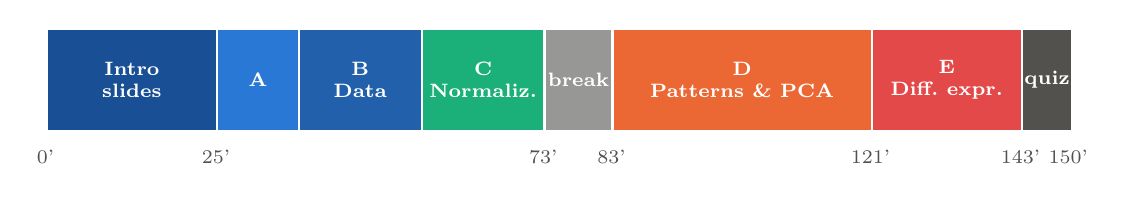
\begin{tikzpicture}[font=\scriptsize, every node/.style={align=center},
      seg/.style={draw=white,thick,minimum height=1.3cm,text=white,font=\scriptsize\bfseries,inner sep=1pt}]
    \def\u{0.0866}   % cm per minute, total width = 150 min = 13 cm
    \node[seg,fill=ucoblue,       minimum width={25*\u cm}, anchor=west] at (0,0)   {Intro\\ slides};
    \node[seg,fill=bluemid,       minimum width={12*\u cm}, anchor=west] at (25*\u,0)  {A};
    \node[seg,fill=bluemid!80!black, minimum width={18*\u cm}, anchor=west] at (37*\u,0)  {B\\ Data};
    \node[seg,fill=greenslot,     minimum width={18*\u cm}, anchor=west] at (55*\u,0)  {C\\ Normaliz.};
    \node[seg,fill=greyink!60,    minimum width={10*\u cm}, anchor=west] at (73*\u,0)  {break};
    \node[seg,fill=orangeslot,    minimum width={38*\u cm}, anchor=west] at (83*\u,0)  {D\\ Patterns \& PCA};
    \node[seg,fill=accentred,     minimum width={22*\u cm}, anchor=west] at (121*\u,0) {E\\ Diff.\ expr.};
    \node[seg,fill=greyink,       minimum width={7*\u cm},  anchor=west] at (143*\u,0) {quiz};
    \foreach \t/\x in {0/0,25/25,73/73,83/83,121/121,143/143,150/150}
      \node[below=0.12cm,text=greyink] at (\x*\u,-0.65) {\t'};
  \end{tikzpicture}

  \vspace{0.35cm}
  \scriptsize
  \begin{tabular}{@{}p{0.05\linewidth}p{0.30\linewidth}p{0.47\linewidth}p{0.10\linewidth}@{}}
    \toprule
    & \textbf{Part} & \textbf{Interactive exercises of the notebook} & \textbf{Time}\\\midrule
    & \textbf{Introduction} (slides) & Python, Jupyter, Colab, RNA-seq, single-cell, pseudobulk, the dataset, AnnData & 25 min\\[1pt]
    \textbf{A} & Python warm-up & 1 Variables $\cdot$ 2 Basic plots & 12 min\\[1pt]
    \textbf{B} & Meet the data & 3 The AnnData object $\cdot$ 4 Distributions: boxplots & 18 min\\[1pt]
    \textbf{C} & Normalization & 5 Raw counts vs CPM $\cdot$ 6 The logarithm & 18 min\\[1pt]
    & \textit{Break} & & 10 min\\[1pt]
    \textbf{D} & Patterns in the data & 7 Heatmaps $\cdot$ 8 PCA: the idea $\cdot$ 9 PCA: all samples $\cdot$ 10 PCA: one cell type & 38 min\\[1pt]
    \textbf{E} & Differential expression & 11 Volcano plots $\cdot$ 12 Comparing two responses & 22 min\\[1pt]
    & Wrap-up and quiz & & 7 min\\
    \bottomrule
  \end{tabular}
\end{frame}

% ════════════════════════════════════════════════════════════════════════════════════════
\section{Introduction}

\begin{frame}[fragile]{What is Python?}
  \begin{columns}[T]
    \begin{column}{0.52\linewidth}
      \begin{itemize}\setlength\itemsep{4pt}
        \item A \alert{general-purpose programming language}: free, readable, with a huge community.
        \item You describe \emph{what to do} step by step, and the computer does it, on 10 or on 10 million samples.
        \item In science it is the \alert{glue} between data and analysis. Packages we use today:
      \end{itemize}
      \small
      \begin{tabular}{@{}ll@{}}
        \code{numpy} & arrays and linear algebra\\
        \code{pandas} & tables\\
        \code{scipy}, \code{statsmodels} & statistics\\
        \code{matplotlib} & plots\\
        \code{scikit-learn} & machine learning\\
        \code{anndata} & omics data containers\\
      \end{tabular}
    \end{column}
    \begin{column}{0.46\linewidth}
\begin{lstlisting}
gene   = "STAT1"          # a variable
counts = 73853            # another one
print(gene, counts)       # show them
\end{lstlisting}
      \vspace{0.15cm}
      \begin{block}{You will not write any code today}
        The notebook gives you \alert{controls} (menus, sliders, boxes) and redraws the figures for you. Your job: \textbf{play, observe, interpret}.
      \end{block}
    \end{column}
  \end{columns}
\end{frame}

\begin{frame}{What is a Jupyter notebook?}
  \begin{columns}[c]
    \begin{column}{0.56\linewidth}
      \centering
      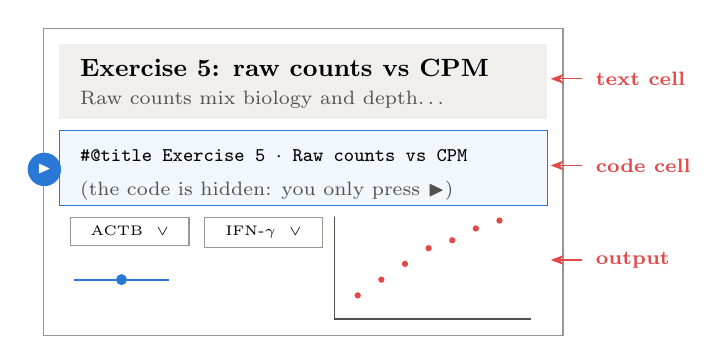
\begin{tikzpicture}[font=\scriptsize, every node/.style={align=left}]
        \node[draw=greyink!60,fill=white,minimum width=6.6cm,minimum height=3.9cm,anchor=north west] (page) at (0,0) {};
        % markdown cell
        \node[draw=none,fill=softgrey,minimum width=6.2cm,minimum height=0.95cm,anchor=north west] (md) at (0.2,-0.2) {};
        \node[anchor=north west,font=\small\bfseries] at (0.35,-0.28) {Exercise 5: raw counts vs CPM};
        \node[anchor=north west,font=\scriptsize,text=greyink] at (0.35,-0.68) {Raw counts mix biology and depth\ldots};
        % code cell
        \node[draw=bluemid,fill=bluemid!6,minimum width=6.2cm,minimum height=0.95cm,anchor=north west] (code) at (0.2,-1.3) {};
        \node[anchor=north west,font=\ttfamily\scriptsize] at (0.35,-1.42) {\#@title Exercise 5 $\cdot$ Raw counts vs CPM};
        \node[anchor=north west,font=\scriptsize,text=greyink] at (0.35,-1.82) {(the code is hidden: you only press $\blacktriangleright$)};
        \node[circle,fill=bluemid,text=white,inner sep=2pt,font=\tiny\bfseries] at (0.02,-1.8) {$\blacktriangleright$};
        % output
        \node[draw=greyink!60,fill=white,minimum width=1.5cm,minimum height=0.3cm,font=\tiny,anchor=north west] at (0.35,-2.4) {ACTB \ $\vee$};
        \node[draw=greyink!60,fill=white,minimum width=1.5cm,minimum height=0.3cm,font=\tiny,anchor=north west] at (2.05,-2.4) {IFN-$\gamma$ \ $\vee$};
        \draw[bluemid,thick] (0.4,-3.2) -- (1.6,-3.2); \fill[bluemid] (1.0,-3.2) circle (0.07);
        \draw[greyink,thin] (3.7,-3.7) -- (3.7,-2.4) -- (3.7,-3.7) -- (6.2,-3.7);
        \foreach \px/\py in {4.0/-3.4,4.3/-3.2,4.6/-3.0,4.9/-2.8,5.2/-2.7,5.5/-2.55,5.8/-2.45} \fill[accentred] (\px,\py) circle (0.04);
        % labels
        \node[anchor=west,text=accentred,font=\scriptsize\bfseries] at (6.9,-0.65) {text cell};
        \node[anchor=west,text=accentred,font=\scriptsize\bfseries] at (6.9,-1.75) {code cell};
        \node[anchor=west,text=accentred,font=\scriptsize\bfseries] at (6.9,-2.95) {output};
        \draw[accentred,-{Stealth}] (6.85,-0.65) -- (6.45,-0.65);
        \draw[accentred,-{Stealth}] (6.85,-1.75) -- (6.45,-1.75);
        \draw[accentred,-{Stealth}] (6.85,-2.95) -- (6.45,-2.95);
      \end{tikzpicture}
    \end{column}
    \begin{column}{0.42\linewidth}\small
      \begin{itemize}\setlength\itemsep{3pt}
        \item A document that mixes \alert{text, code and results}.
        \item Two kinds of cells: \textbf{text} and \textbf{code} (Python). Here the code is \alert{hidden}: a code cell shows only its title.
        \item Run a cell: \alert{$\blacktriangleright$} or \alert{Shift\,+\,Enter}. The output appears below it.
        \item Our outputs are \alert{interactive}: a panel of controls and figures that redraw when you change a control.
        \item A \textbf{kernel} (the Python process behind the notebook) \alert{remembers} what was loaded: run the \textbf{Setup} cell first.
      \end{itemize}
    \end{column}
  \end{columns}
\end{frame}

\begin{frame}{How are we going to run it? Google Colab}
  \begin{columns}[c]
    \begin{column}{0.60\linewidth}
      \centering
      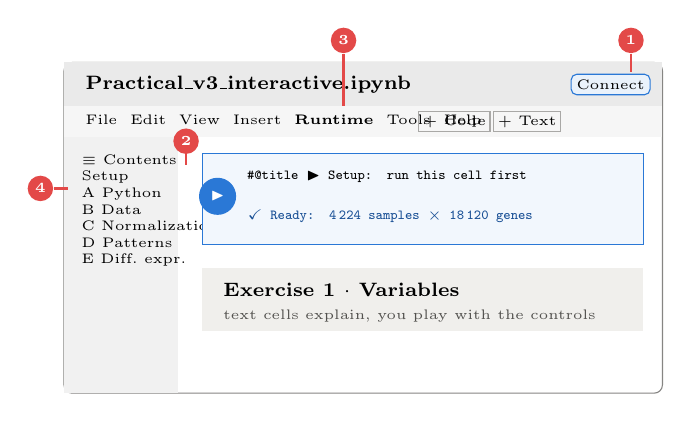
\begin{tikzpicture}[font=\scriptsize, every node/.style={align=left}]
        \draw[rounded corners=3pt,draw=greyink!70,fill=white] (0,0) rectangle (7.6,-4.2);
        \fill[greyink!12] (0,0) rectangle (7.6,-0.55);
        \node[anchor=west,font=\scriptsize\bfseries] at (0.15,-0.28) {Practical\_v3\_interactive.ipynb};
        \node[anchor=east,draw=bluemid,fill=bluemid!10,rounded corners=2pt,inner sep=2pt,font=\tiny] at (7.45,-0.28) {Connect};
        \fill[greyink!5] (0,-0.55) rectangle (7.6,-0.95);
        \node[anchor=west,font=\tiny] at (0.15,-0.75) {File\ \ Edit\ \ View\ \ Insert\ \ \textbf{Runtime}\ \ Tools\ \ Help};
        \node[anchor=west,font=\tiny,draw=greyink!50,inner sep=1.5pt] at (4.5,-0.75) {+ Code};
        \node[anchor=west,font=\tiny,draw=greyink!50,inner sep=1.5pt] at (5.45,-0.75) {+ Text};
        \fill[greyink!8] (0,-0.95) rectangle (1.45,-4.2);
        \node[anchor=north west,font=\tiny] at (0.1,-1.05) {$\equiv$ Contents\\ Setup\\ A Python\\ B Data\\ C Normalization\\ D Patterns\\ E Diff.\ expr.};
        \node[draw=bluemid,fill=bluemid!6,minimum width=5.6cm,minimum height=1.15cm,anchor=north west] at (1.75,-1.15) {};
        \node[anchor=north west,font=\ttfamily\tiny] at (2.2,-1.25) {\#@title $\blacktriangleright$ Setup: run this cell first};
        \node[circle,fill=bluemid,text=white,inner sep=2.5pt,font=\tiny] at (1.95,-1.7) {$\blacktriangleright$};
        \node[anchor=north west,font=\ttfamily\tiny,text=ucoblue] at (2.2,-1.75) {\checkmark\ Ready: 4\,224 samples $\times$ 18\,120 genes};
        \node[draw=none,fill=softgrey,minimum width=5.6cm,minimum height=0.8cm,anchor=north west] at (1.75,-2.6) {};
        \node[anchor=north west,font=\scriptsize\bfseries] at (1.9,-2.68) {Exercise 1 $\cdot$ Variables};
        \node[anchor=north west,font=\tiny,text=greyink] at (1.9,-3.02) {text cells explain, you play with the controls};
        % numbered callouts
        \foreach \n/\x/\y/\tx/\ty in {1/7.2/0.28/7.2/-0.12, 2/1.55/-1.0/1.55/-1.3, 3/3.55/0.28/3.55/-0.55, 4/-0.3/-1.6/0.05/-1.6} {
          \node[circle,fill=accentred,text=white,inner sep=1.5pt,font=\tiny\bfseries] (c\n) at (\x,\y) {\n};
          \draw[accentred,thick] (c\n) -- (\tx,\ty);
        }
      \end{tikzpicture}
    \end{column}
    \begin{column}{0.38\linewidth}\small
      \begin{itemize}\setlength\itemsep{3pt}
        \item Jupyter in your \alert{browser}: nothing to install. Free, with a Google account.
        \item Your code runs on a \alert{temporary computer} in Google's cloud.
      \end{itemize}
      \vspace{0.1cm}
      \begin{enumerate}\setlength\itemsep{2pt}\footnotesize
        \item[\textcolor{accentred}{\textbf{1}}] \textbf{Connect} to a session
        \item[\textcolor{accentred}{\textbf{2}}] $\blacktriangleright$ \textbf{run} a cell
        \item[\textcolor{accentred}{\textbf{3}}] \textbf{Runtime} menu: run all, restart
        \item[\textcolor{accentred}{\textbf{4}}] \textbf{Table of contents}: jump between parts
      \end{enumerate}
    \end{column}
  \end{columns}
\end{frame}

\begin{frame}{How to use the interactive notebook}
  \begin{columns}[c]
    \begin{column}{0.35\linewidth}\footnotesize
      \begin{enumerate}\setlength\itemsep{3pt}
        \item[\textcolor{accentred}{\textbf{1}}] Run the \textbf{Setup} cell first ($\blacktriangleright$): wait for \alert{\checkmark\ Ready} (about 2 min).
        \item[\textcolor{accentred}{\textbf{2}}] In each exercise press $\blacktriangleright$ \alert{once}: the controls appear.
        \item[\textcolor{accentred}{\textbf{3}}] \alert{Change a control}: the figures and tables update by themselves.
        \item[\textcolor{accentred}{\textbf{4}}] Read the \textbf{questions} below, think, and only then open the answer.
      \end{enumerate}
      \vspace{0.05cm}
      \begin{block}{Good to know}
        \scriptsize
        \begin{itemize}\setlength\itemsep{1pt}
          \item \texttt{Ctrl} (\texttt{Cmd} on Mac) \texttt{+ click} selects several items; press \texttt{Enter} after typing.
          \item Something odd? Run the exercise cell again. If the session restarted: Setup again.
          \item Sessions are \alert{temporary}: \textbf{File $\rightarrow$ Save a copy in Drive}.
        \end{itemize}
      \end{block}
    \end{column}
    \begin{column}{0.63\linewidth}
      \centering
      \begin{tikzpicture}
        \node[inner sep=0] (img) {\includegraphics[width=0.97\linewidth]{notebook_ui_ex5.png}};
        \foreach \n/\f in {1/0.03, 2/0.30, 3/0.72} {
          \node[circle,fill=accentred,text=white,inner sep=1.5pt,font=\scriptsize\bfseries] at ($(img.north west)!\f!(img.south west)+(-0.2cm,0)$) {\n};
        }
      \end{tikzpicture}\\[-2pt]
      {\tiny An exercise of the notebook (Exercise 5): controls on top, figures that redraw when you change them.}
    \end{column}
  \end{columns}
\end{frame}

% ────────────────────────────────────────────────────────────────────────────────────────
\begin{frame}{What is transcriptomics via RNA-seq?}
  \centering
  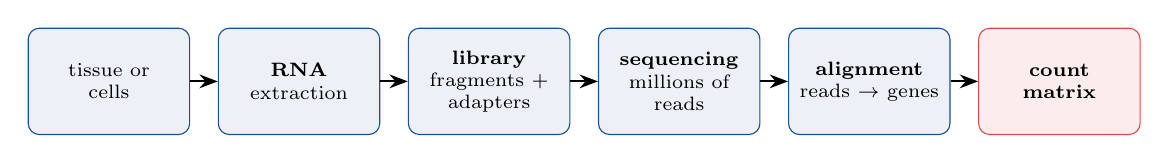
\begin{tikzpicture}[font=\scriptsize, every node/.style={align=center},
      stp/.style={draw=ucoblue,fill=ucoblue!8,rounded corners,minimum height=1.35cm,minimum width=2.05cm,inner sep=2pt}]
    \node[stp] (a) {tissue or\\ cells};
    \node[stp,right=0.35cm of a] (b) {\textbf{RNA}\\ extraction};
    \node[stp,right=0.35cm of b] (c) {\textbf{library}\\ fragments +\\ adapters};
    \node[stp,right=0.35cm of c] (d) {\textbf{sequencing}\\ millions of\\ reads};
    \node[stp,right=0.35cm of d] (e) {\textbf{alignment}\\ reads $\to$ genes};
    \node[stp,right=0.35cm of e,fill=accentred!10,draw=accentred] (f) {\textbf{count}\\ \textbf{matrix}};
    \foreach \x/\y in {a/b,b/c,c/d,d/e,e/f} \draw[-{Stealth},thick] (\x) -- (\y);
  \end{tikzpicture}
  \vspace{0.35cm}

  \begin{columns}[T]
    \begin{column}{0.5\linewidth}\small
      \begin{itemize}\setlength\itemsep{3pt}
        \item The \alert{transcriptome} is the set of all RNA molecules in a sample: which genes are \emph{on}, and how much.
        \item \textbf{Bulk RNA-seq} measures \alert{one average profile per sample}: all cells are mixed.
        \item A \textbf{count} is the number of molecules (or reads) assigned to a gene.
      \end{itemize}
    \end{column}
    \begin{column}{0.46\linewidth}
      \centering\footnotesize
      \begin{tabular}{lrrr}
        \toprule
        gene & sample 1 & sample 2 & sample 3\\\midrule
        \gene{STAT1} & 5\,310 & 12\,874 & 4\,990\\
        \gene{CXCL9} & 12 & 1\,950 & 9\\
        \gene{ACTB} & 36\,500 & 41\,200 & 33\,800\\
        $\vdots$ & $\vdots$ & $\vdots$ & $\vdots$\\
        \bottomrule
      \end{tabular}\\[2pt]
      \scriptsize a count matrix: \alert{genes $\times$ samples} (illustrative numbers)
    \end{column}
  \end{columns}
\end{frame}

\begin{frame}{RNA-seq in three worlds: in vivo, in vitro, in silico}
  \begin{columns}[c]
    \begin{column}{0.54\linewidth}
      \centering\includegraphics[width=\linewidth,height=0.78\textheight,keepaspectratio]{wiki_rnaseq_summary.png}\\[2pt]
      {\tiny Figure: T.\ Shafee, Wikimedia Commons, ``Summary of RNA-Seq'' (CC BY 4.0)}\\[6pt]
      \begin{minipage}{0.92\linewidth}\centering {\scriptsize \textbf{Recommended reading:} visit \href{https://en.wikipedia.org/wiki/RNA-Seq}{\alert{en.wikipedia.org/wiki/RNA-Seq}} for a good overview of the method.}\end{minipage}
    \end{column}
    \begin{column}{0.43\linewidth}\footnotesize
      \begin{itemize}\setlength\itemsep{3pt}
        \item \textbf{In vivo}: the cell \alert{transcribes} a gene into pre-mRNA and splices it into \alert{mature mRNA}. This is what we want to measure.
        \item \textbf{In vitro}: in the lab the RNA is \alert{fragmented}, converted to \alert{cDNA} and \alert{sequenced}, giving millions of short reads.
        \item \textbf{In silico}: the reads are \alert{aligned} to the genome. \alert{Many reads on a gene = highly expressed}, and counting them gives the count matrix.
      \end{itemize}
      \vspace{0.05cm}
      \begin{block}{The key idea}
        We never see the RNA directly: we count \alert{reads} and infer expression from them.
      \end{block}
    \end{column}
  \end{columns}
\end{frame}

\begin{frame}{Bulk and single-cell RNA-seq: the two workflows}
  \begin{columns}[c]
    \begin{column}{0.3\linewidth}
      \centering\includegraphics[width=\linewidth,height=0.8\textheight,keepaspectratio]{tzec_fig1_bulk.png}
    \end{column}
    \begin{column}{0.3\linewidth}
      \centering\includegraphics[width=\linewidth,height=0.8\textheight,keepaspectratio]{tzec_fig2_sc.png}
    \end{column}
    \begin{column}{0.36\linewidth}\small
      \begin{itemize}\setlength\itemsep{4pt}
        \item Same logic, different unit: a \alert{sample} (bulk) or a \alert{cell} (single-cell).
        \item Both end in a \alert{count matrix}, which is then normalized and analysed (differential expression, enrichment\ldots).
        \item Single-cell adds \alert{barcoding} to trace each read to its cell, and quality control per cell.
      \end{itemize}
      {\tiny Figures 1 and 2 of Tzec-Interi\'an \emph{et al.}\ 2025, \emph{Quant.\ Biol.}\ (CC BY)}
    \end{column}
  \end{columns}
\end{frame}

\begin{frame}{Single-cell transcriptomics: one profile per cell}
  \begin{columns}[c]
    \begin{column}{0.5\linewidth}
      \centering
      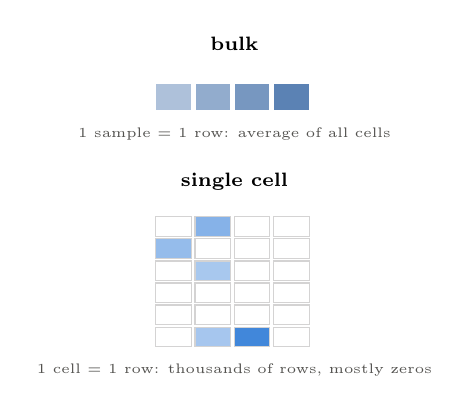
\begin{tikzpicture}[font=\scriptsize, every node/.style={align=center}]
        % bulk
        \node[font=\scriptsize\bfseries] at (1.0,2.6) {bulk};
        \foreach \c in {0,...,3} { \fill[ucoblue!\the\numexpr 35+\c*12\relax,draw=white] (\c*0.5,2.1) rectangle ++(0.45,-0.35); }
        \node[font=\tiny,text=greyink] at (1.0,1.45) {1 sample = 1 row: average of all cells};
        % single cell
        \node[font=\scriptsize\bfseries] at (1.0,0.85) {single cell};
        \foreach \r in {0,...,5} {
          \foreach \c in {0,...,3} {
            \pgfmathsetmacro{\v}{ifthenelse(rnd>0.72,rnd*65+35,0)}
            \fill[bluemid!\v!white,draw=greyink!25] (\c*0.5,0.4-\r*0.28) rectangle ++(0.45,-0.25);
          }
        }
        \node[font=\tiny,text=greyink] at (1.0,-1.55) {1 cell = 1 row: thousands of rows, mostly zeros};
      \end{tikzpicture}
    \end{column}
    \begin{column}{0.48\linewidth}\small
      \begin{tabular}{@{}>{\raggedright\arraybackslash}p{0.2\linewidth}>{\raggedright\arraybackslash}p{0.25\linewidth}>{\raggedright\arraybackslash}p{0.45\linewidth}@{}}
        \toprule
        & \textbf{bulk} & \textbf{single-cell}\\\midrule
        unit & sample & cell\\
        rows & tens & $10^4$--$10^7$\\
        zeros & few & most entries\\
        reveals & average & cell types and rare cells\\
        \bottomrule
      \end{tabular}
      \vspace{0.25cm}
      \begin{itemize}\footnotesize\setlength\itemsep{3pt}
        \item Every cell gets a \alert{barcode}, so reads can be traced back to their cell.
        \item Cell types are then identified by clustering and \emph{marker genes} (e.g.\ \gene{LYZ} for monocytes, \gene{CD3E} for T cells).
      \end{itemize}
    \end{column}
  \end{columns}
\end{frame}

\begin{frame}{Single-cell by combinatorial indexing (split-pool barcoding)}
  \centering
  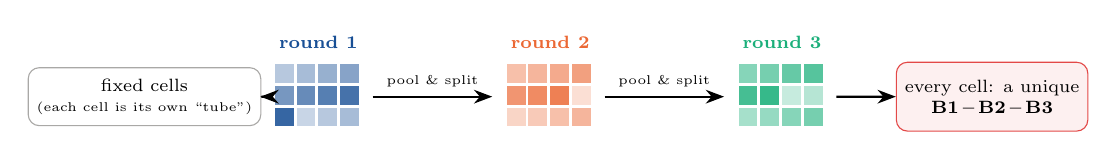
\begin{tikzpicture}[scale=0.92,transform shape,font=\scriptsize, every node/.style={align=center}]
    % plates: 3 small grids
    \foreach \p/\x/\col in {1/0.3/ucoblue, 2/3.5/orangeslot, 3/6.7/greenslot} {
      \foreach \r in {0,...,2} \foreach \c in {0,...,3} {
        \pgfmathsetmacro{\sh}{20+mod((\r*4+\c)*7+\p*11,70)}
        \fill[\col!\sh!white] (\x+\c*0.3,-\r*0.3) rectangle ++(0.26,-0.26);
      }
      \node[font=\scriptsize\bfseries,text=\col] at (\x+0.6,0.3) {round \p};
    }
    \node[draw=greyink!50,rounded corners,minimum width=1.9cm,minimum height=0.8cm,font=\scriptsize] (cells) at (-1.5,-0.45) {fixed cells\\ \tiny (each cell is its own ``tube'')};
    \draw[-{Stealth},thick] (cells) -- (0.1,-0.45);
    \draw[-{Stealth},thick] (1.65,-0.45) -- node[above,font=\tiny] {pool \& split} (3.3,-0.45);
    \draw[-{Stealth},thick] (4.85,-0.45) -- node[above,font=\tiny] {pool \& split} (6.5,-0.45);
    \node[draw=accentred,fill=accentred!8,rounded corners,minimum width=2.5cm,minimum height=0.95cm] (res) at (10.2,-0.45) {every cell: a unique\\ \textbf{B1\,--\,B2\,--\,B3}};
    \draw[-{Stealth},thick] (8.05,-0.45) -- (res);
  \end{tikzpicture}
  \vspace{0.3cm}

  \begin{columns}[T]
    \begin{column}{0.54\linewidth}\small
      \begin{itemize}\setlength\itemsep{3pt}
        \item In each round the cells are \alert{distributed in wells at random}; every well adds its own barcode to the RNA of the cells inside it.
        \item After three rounds the chance that two cells share the same three barcodes is tiny: with 96 barcodes per round, $96^3\approx 880\,000$ combinations (illustrative).
        \item \textbf{No droplets, no cell isolation}: millions of cells in one experiment.
      \end{itemize}
    \end{column}
    \begin{column}{0.42\linewidth}
      \begin{block}{In our data}
        \footnotesize
        The \alert{first-round barcode} is the well of the stimulation plate, i.e.\ the \alert{condition}: donor $\times$ cytokine. It is the \code{bc1\_well} column of the raw file.\\[2pt]
        The PBS control was spread over \alert{6 wells}.
      \end{block}
    \end{column}
  \end{columns}
\end{frame}

\begin{frame}{Why do we need to pseudobulk first?}
  \centering
  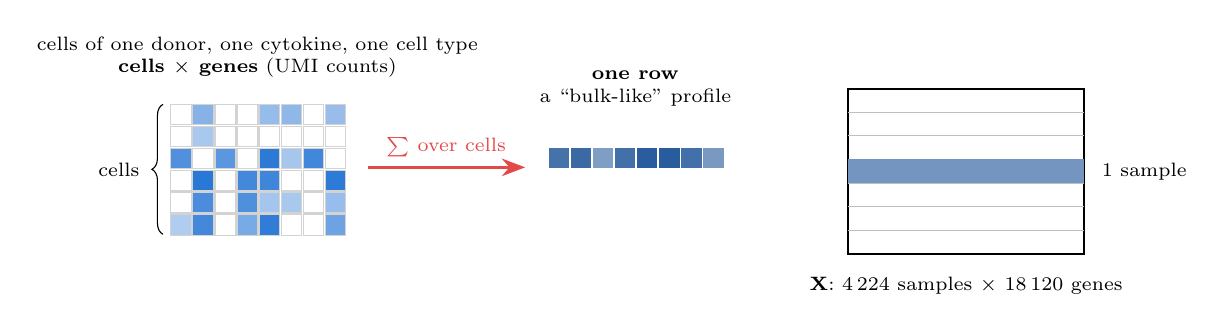
\begin{tikzpicture}[font=\scriptsize]
    \foreach \r in {0,...,5} {
      \foreach \c in {0,...,7} {
        \pgfmathsetmacro{\v}{ifthenelse(rnd>0.5,rnd*65+35,0)}
        \fill[bluemid!\v!white,draw=greyink!25] (\c*0.28,-\r*0.28) rectangle ++(0.26,-0.26);
      }
    }
    \node[align=center] at (1.1,0.6) {cells of one donor, one cytokine, one cell type\\ \textbf{cells $\times$ genes} (UMI counts)};
    \draw[decorate,decoration={brace,amplitude=4pt,mirror}] (-0.1,0) -- (-0.1,-1.65) node[midway,left=5pt] {cells};
    \draw[-{Stealth},very thick,accentred] (2.5,-0.8) -- node[above] {$\sum$ over cells} (4.5,-0.8);
    \foreach \c in {0,...,7} {
      \pgfmathsetmacro{\v}{rnd*45+50}
      \fill[ucoblue!\v] (4.8+\c*0.28,-0.55) rectangle ++(0.26,-0.26);
    }
    \node[align=center] at (5.9,0.2) {\textbf{one row}\\ a ``bulk-like'' profile};
    \draw[thick] (8.6,0.2) rectangle (11.6,-1.9);
    \foreach \r in {1,...,6} \draw[gray!50] (8.6,0.2-0.3*\r) -- (11.6,0.2-0.3*\r);
    \fill[ucoblue!60] (8.6,-0.7) rectangle (11.6,-1.0);
    \node[right] at (11.7,-0.85) {1 sample};
    \node at (10.1,-2.3) {\textbf{X}: \numnsamples\ samples $\times$ \numngenesraw\ genes};
  \end{tikzpicture}
  \vspace{0cm}

  \begin{itemize}\small\setlength\itemsep{2pt}
    \item \alert{The unit of replication is the donor, not the cell}: millions of cells come from only 12 people, and cells of one person are not independent. Testing cells as if they were replicates gives many false positives (\emph{pseudoreplication}).
    \item Single-cell counts are sparse and noisy; summed over thousands of cells they behave like \alert{bulk RNA-seq}, so standard, transparent statistics apply.
    \item It makes the data small: 9.7 million cells $\to$ \numnsamples\ samples.
  \end{itemize}
\end{frame}

% ────────────────────────────────────────────────────────────────────────────────────────
\begin{frame}{The dataset: the Human Cytokine Dictionary}
  \begin{columns}[c]
    \begin{column}{0.52\linewidth}
      \centering
      \includegraphics[width=\linewidth,height=0.74\textheight,keepaspectratio]{paper_fig1ab.png}\\[-1pt]
      {\tiny Oesinghaus \emph{et al.}\ 2025, Fig.\ 1a--b (CC BY-NC-ND 4.0)}
    \end{column}
    \begin{column}{0.44\linewidth}\small
      \begin{itemize}\setlength\itemsep{4pt}
        \item \alert{12 healthy donors} (6 female, 6 male; 34--75 years)
        \item \alert{90 cytokines} + a PBS control, in vitro for \alert{24 h}
        \item $\sim$\alert{9.7 million} PBMCs after quality control
        \item 16 cell types, annotated by marker genes (panel b)
      \end{itemize}
      \vspace{0.2cm}
      \footnotesize
      \textbf{Question of the paper:} what does every cytokine do to every immune cell type, and how much do people differ?
    \end{column}
  \end{columns}
\end{frame}

\begin{frame}{How the data were generated}
  \centering
  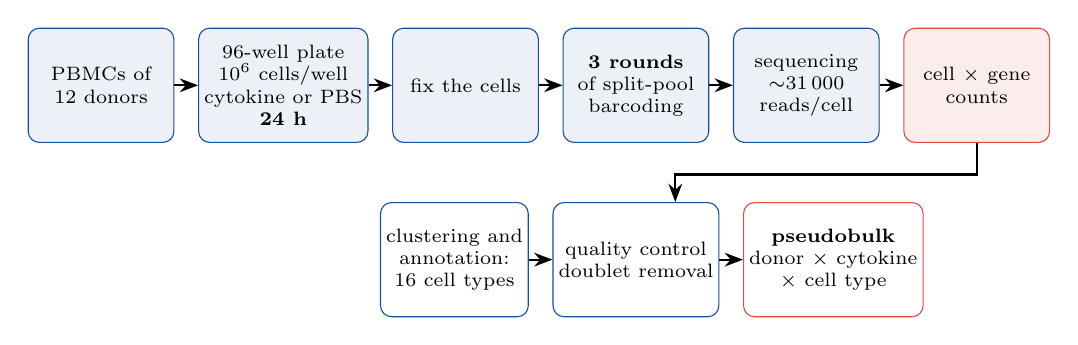
\begin{tikzpicture}[font=\scriptsize, every node/.style={align=center},
      stp/.style={draw=ucoblue,fill=ucoblue!8,rounded corners,minimum height=1.45cm,minimum width=1.85cm,inner sep=2pt},
      numdot/.style={circle,fill=accentred,text=white,inner sep=1.5pt,font=\tiny\bfseries}]
    \node[stp] (a) {PBMCs of\\ 12 donors};
    \node[stp,right=0.3cm of a] (b) {96-well plate\\ 10$^6$ cells/well\\ cytokine or PBS\\ \textbf{24 h}};
    \node[stp,right=0.3cm of b] (c) {fix the cells};
    \node[stp,right=0.3cm of c] (d) {\textbf{3 rounds}\\ of split-pool\\ barcoding};
    \node[stp,right=0.3cm of d] (e) {sequencing\\ $\sim$31\,000\\ reads/cell};
    \node[stp,right=0.3cm of e,fill=accentred!10,draw=accentred] (f) {cell $\times$ gene\\ counts};
    \foreach \x/\y in {a/b,b/c,c/d,d/e,e/f} \draw[-{Stealth},thick] (\x) -- (\y);
    \node[stp,below=0.75cm of d,fill=white] (g) {quality control\\ doublet removal};
    \node[stp,left=0.3cm of g,fill=white] (h) {clustering and\\ annotation:\\ 16 cell types};
    \node[stp,right=0.3cm of g,fill=white,draw=accentred] (i) {\textbf{pseudobulk}\\ donor $\times$ cytokine\\ $\times$ cell type};
    \draw[-{Stealth},thick] (f.south) |- ($(g.north)+(0.5,0.35)$) -- ($(g.north)+(0.5,0)$);
    \draw[-{Stealth},thick] (g) -- (i); \draw[-{Stealth},thick] (h) -- (g);
  \end{tikzpicture}
  \vspace{0.25cm}

  \footnotesize
  \begin{itemize}\setlength\itemsep{2pt}
    \item Barcoding with the Parse Biosciences GigaLab protocol; sublibraries of $\sim$100\,000 cells; sequencing on an Ultima UG-100.
    \item Cells kept with 400--7\,000 detected genes and $<15\,\%$ mitochondrial reads.
  \end{itemize}
\end{frame}

\begin{frame}{What is in the subset we work with?}
  \begin{columns}[T]
    \begin{column}{0.56\linewidth}
      \small
      \begin{tabular}{@{}>{\raggedright\arraybackslash}p{0.2\linewidth}>{\raggedright\arraybackslash}p{0.22\linewidth}>{\raggedright\arraybackslash}p{0.52\linewidth}@{}}
        \toprule
        & \textbf{paper} & \textbf{our practical}\\\midrule
        donors & 12 & 12\\[1pt]
        cytokines & 90 + PBS & 87 + PBS\\[1pt]
        cell types & 16 & 4: CD4 T, CD8 T, NK CD56\textsuperscript{low}, CD14 monocytes\\[1pt]
        unit & single cells & \alert{pseudobulk} samples\\[1pt]
        genes & all & \numngenesraw\ protein-coding ($\to$ \numngenes\ after filtering)\\
        \bottomrule
      \end{tabular}
    \end{column}
    \begin{column}{0.4\linewidth}
      \begin{block}{The design}
        \centering
        $4$ cell types\\ $\times$ $88$ conditions\\ \footnotesize(87 cytokines + PBS)\\ \normalsize $\times$ $12$ donors\\[3pt]
        $=$ \alert{\numnsamples\ samples}
      \end{block}
      \footnotesize
      The PBS control was measured in 6 wells; the file stores each well \emph{and} their total. We keep the total.
    \end{column}
  \end{columns}
\end{frame}

\begin{frame}{AnnData: a Python data structure for omics data}
  \begin{columns}[c]
    \begin{column}{0.38\linewidth}
      \centering
      \includegraphics[width=\linewidth,height=0.76\textheight,keepaspectratio]{anndata_schema.png}\\[-1pt]
      {\tiny AnnData schema (anndata documentation)}
    \end{column}
    \begin{column}{0.58\linewidth}\small
      \begin{itemize}\setlength\itemsep{3pt}
        \item \textbf{One object, several tables that always stay aligned.}
        \item \textcolor{ucoblue}{\textbf{\code{X}}}: the main matrix, $n_{\text{obs}}\times n_{\text{vars}}$
        \item \textcolor{yellowslot}{\textbf{\code{obs}}}: one row per \alert{observation} (sample or cell): metadata
        \item \textcolor{bluemid}{\textbf{\code{var}}}: one row per \alert{variable} (gene): metadata
        \item \textcolor{greenslot}{\textbf{\code{layers}}}: more matrices, same shape as \code{X}
        \item \code{obsm}, \code{varm}, \code{obsp}, \code{varp}, \code{uns}: embeddings (PCA), graphs, free-form results
      \end{itemize}
      \vspace{0.15cm}
      \begin{block}{Why it matters}
        \footnotesize Subsetting moves \emph{all} the tables together: no gene or sample can get out of sync with its metadata. Saved as an \code{.h5ad} file.
      \end{block}
    \end{column}
  \end{columns}
\end{frame}

\begin{frame}[fragile]{AnnData in our practical}
  \begin{columns}[T]
    \begin{column}{0.52\linewidth}
      \small
      \begin{tabular}{@{}>{\ttfamily}p{0.16\linewidth}>{\raggedright\arraybackslash}p{0.47\linewidth}>{\raggedright\arraybackslash}p{0.3\linewidth}@{}}
        \toprule
        \textrm{\textbf{slot}} & \textbf{our data} & \textbf{shape}\\\midrule
        X & raw counts & \numnsamples\,$\times$\,\numngenesraw\\[2pt]
        obs & donor, cytokine, treatment, cell\_type, number of cells, library size & \numnsamples\ rows\\[2pt]
        var & gene names, total counts, samples where detected & \numngenesraw\ rows\\[2pt]
        layers & \code{cpm}, \code{log2cpm} (normalized versions) & same as \code{X}\\
        \bottomrule
      \end{tabular}
    \end{column}
    \begin{column}{0.46\linewidth}
\begin{lstlisting}
# rows first (samples), then genes
adata[["Donor1|CD14_Mono|IFN-gamma"],
      ["STAT1"]]

mask = adata.obs["cell_type"] == "CD14_Mono"
adata[mask, ["IDO1", "CXCL10"]]
\end{lstlisting}
      \footnotesize The first selection is $1\times1$; the second one, $1\,056\times2$ (all monocyte samples). In the notebook (Exercise 3) you build such subsets with \alert{menus}, no code.
    \end{column}
  \end{columns}
  \vspace{0.25cm}
  \begin{block}{Hands-on}
    \small Back to the notebook: run the \textbf{Setup} cell (install, download and prepare the data), then start with \textbf{Exercise 1}.
    \timebox{about 25 min for the introduction}
  \end{block}
\end{frame}


% ════════════════════════════════════════════════════════════════════════════════════════
\begin{frame}{Quick quiz: 3 questions}
  \begin{columns}[T]
    \begin{column}{0.62\textwidth}
      \large Open \href{https://apps.garridolab.org/quiz/}{\alert{\texttt{apps.garridolab.org/quiz/}}}
      \normalsize\vspace{0.3cm}

      \begin{enumerate}\setlength\itemsep{6pt}
        \item Log in with your \alert{UCO email}. The login appears when the quiz is opened (at the end of the practical).
        \item You get \alert{3 random questions} about the practical: one correct answer each.
        \item You can submit \alert{only once}. You will see your score right away.
      \end{enumerate}
    \end{column}
    \begin{column}{0.34\textwidth}
      \centering
      \qrcode[height=3.6cm]{https://apps.garridolab.org/quiz/}\\[4pt]
      \scriptsize scan with your phone
    \end{column}
  \end{columns}
\end{frame}

\appendix
\begin{frame}{References}
  \scriptsize
  \begin{itemize}\setlength\itemsep{3pt}
    \item Oesinghaus L.\ \emph{et al.} (2025) A single-cell cytokine dictionary of human peripheral blood. \emph{bioRxiv}. \texttt{doi:10.64898/2025.12.12.693897}
    \item Virshup I.\ \emph{et al.} (2024) anndata: Access and store annotated data matrices. \emph{J.\ Open Source Softw.} 9(101):4371.
    \item Heumos L.\ \emph{et al.} (2023) Best practices for single-cell analysis across modalities. \emph{Nat.\ Rev.\ Genet.} 24:550--572.
    \item Tzec-Interi\'an J.A., Gonz\'alez-Padilla D., G\'ongora-Castillo E.B. (2025) Bioinformatics perspectives on transcriptomics: a comprehensive review of bulk and single-cell RNA sequencing analyses. \emph{Quant.\ Biol.} e78. \texttt{doi:10.1002/qub2.78}
    \item Squair J.W.\ \emph{et al.} (2021) Confronting false discoveries in single-cell differential expression. \emph{Nat.\ Commun.} 12:5692.
    \item Love M.I., Huber W., Anders S. (2014) Moderated estimation of fold change and dispersion for RNA-seq data with DESeq2. \emph{Genome Biol.} 15:550.
    \item Muzellec B.\ \emph{et al.} (2023) PyDESeq2: a python package for bulk RNA-seq differential expression analysis. \emph{Bioinformatics} 39:btad547.
    \item Benjamini Y., Hochberg Y. (1995) Controlling the false discovery rate. \emph{J.\ R.\ Stat.\ Soc.\ B} 57:289--300.
  \end{itemize}
\end{frame}

\end{document}
